\section*{Ergebnisse}
\label{sec:Ergebnisse}

Entsprechend dem Kaiser-Kriterium für signifikante Faktoren ab einem Eigenwert von mindestens 1 erstellt die Faktorenanalyse aus den 13 von Probanden bewerteten Attributen vier Faktoren.
Das Kaiser-Meyer-Olkin-Kriterium der Faktorenanalyse nimmt einen Wert von 0,734 an, was einem ziemlich guten Ausmaß an Interkorrelation zwischen den Variablen entspricht \cite{eckey2002multivariate}.
Die vier Faktoren decken insgesamt 67\% der Gesamtvarianz.
Wenige Variablen laden dabei mit einer Faktorladung von mindestens 0,66 relativ stark in einen Faktor, während sie gleichzeitig mit einem maximalen Wert von 0,46 eher schwach in die übrigen Faktoren laden.
Einzig die Variable \textit{Emotional} lädt in keines der Faktoren stark und entfällt aus diesem Grund aus der inhaltlichen Beschreibung der erzeugten Faktoren.
Die vier erzeugten Faktoren werden inhaltlich gekennzeichnet als \textit{Ruhig} für den 1. Faktor, \textit{Niveauvoll} für den 2. Faktor, \textit{Heiter} für den 3. Faktor und \textit{Energisch} für den 4. Faktor (vgl. Tabelle \ref{tab:faktoren}).   


\begin{table}[htbp]
    \centering
    \caption{Faktoren}
    \vspace{2mm}
    \label{tab:faktoren}
        \begin{tabularx}{8.4cm}{|X|X|X|X|}
            \hline Faktor 1: \textbf{Ruhig} & Faktor 2: \textbf{Niveauvoll} & Faktor 3: \textbf{Heiter} & Faktor 4: \textbf{Energisch} \\
            \hline Entspan\-nend & Anspruchs\-voll       & Fröhlich             & Erregend \\
            \hline Warm              & Komplex                  & - Traurig            & Intensiv \\
            \hline Sanft               & - Einfach                 & Tanzbar             & \\
            \hline                        & Intellek\-tuell          &                          & \\
            \hline
        \end{tabularx}
\end{table}


Die Regressionen dieser Faktoren mit den Features von Spotify liefern Modelle mit sehr hohen Signifikanzen nahe 0 (vgl. Tabelle 1).
Als Kriterium für das Aufnehmen einer Variable für ein Modell ist ein maximaler Signikanzwert von  0,05.  
Das Modell mit der höchsten Güte erhalten wir bei der Regression mit dem Faktor \textit{Heiter}.
23,1\% der Varianz wird vom Modell, dass die Variablen \textit{SP\_danceability}, \textit{SP\_energy}, \textit{SP\_instrumentalness} und \textit{SP\_valence} enthält, gedeckt.
Die Variable \textit{SP\_energy} ist in dem Modell am stärksten gewichtet, gefolgt von den Variablen \textit{SP\_danceability},  \textit{SP\_instrumentalness} und \textit{SP\_valence}.
Das Streudiagramm dieser Regression ist in Abb. \ref{fig:Faktor3} zu sehen.    
Ein Modell mit einer ähnlich hohem Bestimmtheitsmaß R-quadrat gibt die Regression mit dem Faktor \textit{Ruhig} aus, die 21,5\% der Varianz gedeckt.
Enthalten in diesem Modell ist die Variable \textit{SP\_energy}, die mit einer negativen Effektstärke etwa vier mal stärker gewichtet ist als die zweite in dem Modell enthaltenen Variable \textit{SP\_speechiness}.
Deutlich schlechtere Modellanpassungen liefert die Regressionen mit den Faktoren \textit{Niveauvoll} und \textit{Energisch}.
Wir erhalten ein Modell mit einer Güte von 0,112 bei der Regression mit dem Faktor \textit{Energisch} und nur 0,038 bei der Regression mit dem Faktor \textit{Niveauvoll}.

\begin{table}[htbp]
    \centering
    \caption{Ergebnisse der Regressionen}
    \vspace{2mm}
    \label{tab:DescriptiveTextForATable}
        \begin{tabularx}{8,4cm}{@{\extracolsep{\fill}} @{\arrayrulewidth1.5pt\vline}c@{\arrayrulewidth1.5pt\vline}Y|l|l|l@{\arrayrulewidth1.5pt\vline}}
            \noalign{\hrule height1.5pt}
            Faktor & Modell & Beta & Sig. & $\text{R}^2$ \\
            \noalign{\hrule height1.5pt}
            \multirow{2}{*}{Ruhig}  & energy & -0,434 & 0,000 & \multirow{2}{*}{0,215} \\
                \cline{2-4}
                & speechiness & -0,100 & 0,040 & \\
            \noalign{\hrule height1.5pt}
            \multirow{2}{*}{Niveauvoll} & instrumentalness & 0,130 & 0,020 & \multirow{2}{*}{0,038} \\
                \cline{2-4}
                & loudness & -0,110 & 0,048 & \\
                \noalign{\hrule height1.5pt}
            \multirow{4}{*}{Heiter} & danceability & 0,247 & 0,000 & \multirow{4}{*}{0,231} \\
                \cline{2-4}
                & energy & 0,279 &  0,000 & \\
                \cline{2-4}
                & instrumentalness & 0,204 & 0,000 & \\
                \cline{2-4}
                & valennce & 0,136 & 0,021 & \\
                \noalign{\hrule height1.5pt}
            \multirow{3}{*}{Energisch} & valence & -0,238 & 0,000 & \multirow{3}{*}{0,112} \\
                \cline{2-4}
                & loudness & 0,287 & 0,000 & \\
                \cline{2-4}
                & instrumentalness & 0,139 & 0,010 & \\
            \noalign{\hrule height1.5pt}
        \end{tabularx}
\end{table}

\begin{figure}[hbt]
    \begin{center}
        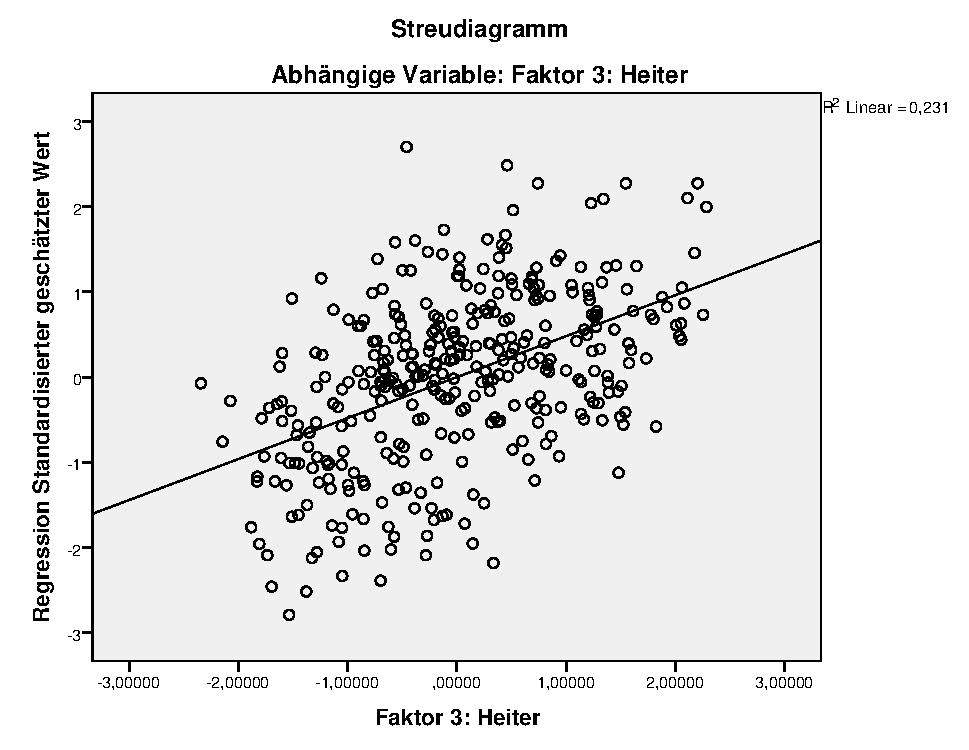
\includegraphics[width=8cm]{images/StreudiagrammFak3.pdf}
    \end{center}
    \caption{Streudiagramm und Regressionsgerade der Regression mit dem Faktor \textit{Heiter}. Diese liefert die beste Modellanpassung.}
    \label{fig:Faktor3}
\end{figure}

\section*{Diskussion}
\label{sec:Diskussion}


Die Modelle der Regressionen sind hochsignifikant.
Somit ist ein Zusammenhang zwischen den Bewertungen der Probanden und den Features von Spotify vorhanden.
Die Effektstärken der Modelle sind dagegen eher gering. 
Der höchste Korrelationskoeffizient von 0,481 ist bei der Regression mit dem Faktor \textit{Heiter} vorzufinden. Die weiteren drei Regressionen liefern noch kleinere Korrelationswerte.
Die Deutung der Korrelationswerte der erstellten Modelle auf die Faktoren von dem Datensatz ``10 Songs für die Insel'' deckt sich auch mit der Interpretation von Effektstärken von Cohen.
Dabei entspricht der Korrelationswert r für die Regression mit dem Faktor \textit{Niveauvoll} einem kleinen Effekt, die übrigen entsprechen einem mittleren Effekt. 
Ein starker Effekt, der bei einem Korrelationswert von mindestens 0,5 vorzufinden ist, wird nicht erreicht \cite{cohen1988}.
Somit kann die in der Hypothese formulierte Annahme einer starken Korrelation der Datensätze mit einem Wert von mindestens 0,5 nicht bestätigt werden. 

Die Ergebnisse zeigen, dass die MIR Verfahren von Spotify zur Bewertung von Musikstücken noch Verbesserungspotential haben.
Jedoch sind auch beim Datensatz ``10 Songs für die Insel'' Fehler zu erwarten, die in einen kleineren Korrealtionskoeffizienten resultieren könnten.
Die Songs wurden jeweils nur einmal von nur einer Person bewertet.
Hinzu kommt, dass die Probanden einen besonderen, persönlichen Bezug zu den von ihnen bewerteten Musikstücken haben.
Eine höhere Anzahl an Bewertungen eines einzelnen Musikstücks durch mehrere Probanden mit anschließender Mittelung würden die in diesem Datensatz vorhandenen Fehler minimieren.

Ein weiterer Grund für die geringe Korrelation könnte aber auch die inhaltlich meist nicht direkt entsprechenden Bewertungskriterien beider Datensätze sein.
Es gibt beispielsweise für den Faktor, mit dem schwächsten Korrelationswert, \textit{Niveauvoll} kein Spotify Feature, das diesem Faktor inhaltlich zugeordnet werden kann.
Dahingegen lässt sich eine starke negative Korrelation des Spotify Features \textit{SP\_energy} mit dem Faktor \textit{Ruhig} inhaltlich sinnvoll erschließen.
Gleiches gilt auch für die Korrelation der Features \textit{SP\_danceability}, \textit{SP\_energy}, \textit{SP\_instrumentalness} und \textit{SP\_valence} mit dem Faktor \textit{Heiter}.
Jedoch wurde eine größere Abhängigkeit dieser inhaltlich ähnlichen Variablen, vor allem \textit{SP\_danceability} und \textit{SP\_valence} mit dem Faktor \textit{Heiter} erwartet.
Die Spotify Features \textit{SP\_tempo}, \textit{SP\_liveness}, sowie \textit{SP\_acousticness} korrelieren dagegen nicht signifikant mit einem der Faktoren und werden in keinem Modell aufgenommen. 
Das Feature \textit{SP\_tempo} beschreibt, wie die schon im vorhinein von der Analyse nicht berücksichtigten Features von Spotify, eher die Struktur eines Musikstücks und ähnelt inhaltlich somit keinem der subjektiver Empfindungen entsprechenden Bewertungen aus dem Datensatz ``10 Songs für die Insel''.
\textit{SP\_liveness} und \textit{SP\_acousticness} entsprechen inhaltlich ebenfalls keinem der ``Insel''-Variablen.  

Eine neue empirische Studie, bei der die in dem Datensatz ``10 Songs für die Insel'' vorzufindenden Bewertungskriterien für Musikstücke durch die Spotify Features ersetzt werden würde damit zu einem aussagekräftigerem Ergebnis führen.



